\documentclass[conference,10pt]{IEEEtran}
\IEEEoverridecommandlockouts
\usepackage[utf8]{inputenc}
\usepackage{lastpage}
\usepackage{newtxtext,newtxmath}
\usepackage[dvipsnames,svgnames,x11names,hyperref]{xcolor}
\usepackage[T1]{fontenc}
\usepackage[english]{babel}
\usepackage{array}
\usepackage{url}
\usepackage{graphicx}
\usepackage{flushend}
\usepackage{cite}
\usepackage{algorithmic}
\usepackage[caption=false]{subfig}
\usepackage{hyperref}
\usepackage{microtype}
\usepackage{minted}

\def\UrlBreaks{\do\/\do-}

\newcommand{\papertitle}{SenSQL: Networked Storage and Query Processing Architecture for Spatiotemporal Sensor Data}

% Potential venues for publication:
%
% IFIP Networking 2021 (~ 23\%)
%  * Deadlines:
%    - Abstract: January 5, 2021 (https://edas.info/N27861)
%    - Paper: January 12, 2012
%  * Guidelines:
%    - 9 pages maximum
%    - double-blind review
%
% IEEE DCOSS 2021 (~ 25-30\%)
%  * Deadlines:
%    - Abstract: January 18, 2021 ( https://edas.info/newPaper.php?c=27882)
%    - Paper: January 25, 2021
%  * Guidelines:
%    - 8 pages maximum (2 additional at $100/page for appendices, theorems, implementation)
%    - single-blind review
%
% Usenix ATC 21
%  * Deadlines:
%    - Paper: January 12, 2021
%  * Guidelines:
%    - 11/5 pages maximum (without references)
%    - double-blind review

\hypersetup{
  colorlinks=true,% Color URLs with urlcolor
  linkcolor=black,% The color for internal (cross-reference) links
  urlcolor=Blue4,% The color for URLs (hyperlinks)
  citecolor=black,
  pdftitle={\papertitle}
}

\urlstyle{same}

\begin{document}
\title{\papertitle}

\author{
  \IEEEauthorblockN{
    \href{mailto:janakj@cs.columbia.edu}{\color{black}Jan Janak},
    \href{mailto:hgs@cs.columbia.edu}{\color{black}Henning Schulzrinne}
  }
  \IEEEauthorblockA{
    Department of Computer Science, Columbia University, New York, USA
  }
  Email: \{janakj,hgs\}@cs.columbia.edu
}

\maketitle

\begin{abstract}
TBD
\end{abstract}

\section{Introduction}
\label{sec:introduction}

A cornerstone of every Internet of Things (IoT) system is its data acquisition infrastructure in the form of sensors. Sensors perform measurements and generate data representing measured quantities. The data is then used by applications that monitor on control the system. Some applications require a history of sensor measurements to function, e.g., to calculate aggregates or estimate trends. With the growing size and complexity of IoT systems, the need for a distributed sensor database with a generic query interface arises. Ideally, the database would be application-agnostic with a declarative query interface allowing the programmer to focus on what sensor data to get, rather than how to get it.

We propose a distributed SQL-based storage and query processor architecture for heterogeneous IoT systems. Our architecture provides the application programmer with a familiar declarative SQL query interface to spatiotemporal sensor data that is geographically partitioned and distributed.

This work is part of our broader research effort to develop fundamental programming abstractions for heterogeneous IoT systems.

% Background
%  - introduce classes of sensors
%  - introduce device roles (e.g., storage node)
%  - SELECT-FROM-WHERE-GROUP BY-HAVING-ORDER BY-LIMIT

% Motivation
% - Limit bandwidth, allow sensors generate measurements frequently, transfer only when necessary
% - Compute aggregates close to the source of the data
% - Make aggregation a generic operation that can operate on any data
% - Support intuitive declarative-style interface for application programmers
% - Data functionality partitioning (for reliability purposes)
%
% Data Model

% aggregates
%  - data reduction mechanism
%  - summarization (e.g., for privacy)
%
% SQL is loosely based on a relational algebra
%
% Architecture
% - stateless versus stateful sensors
% - storage node
% - independent sensor system (associated with an administrative entity, a.k.a. principal)
% - service region
% - independent sensor system directory/router
%

\section{Related Work}
\label{sec:related-work}

% Declarative query languages: SQL/MM, GraphQL, GeoSPARQL

% TinyDB: Cite the main (long) TinyDB paper and perhaps some of the earlier related papers
TinyDB \cite{madden2005tinydb} is a distributed query processor for ad hoc sensor networks. Similar to our work, TinyDB provides a generic SQL-like query interface for sensor data to applications. Unlike our architecture, TinyDB does not support spatial predicates, is designed to operate in a uniform environment, and its SQL dialect provides domain-specific primitives for ad hoc sensor networks, e.g., to control measurement data acquisition on energy constrained devices. The obvious drawback of acquisitional query processing is that data is only collected on demand, making it impossible to execute future queries over a history of samples.

Cougar \cite{yao2002cougar} was a similar distributed database architecture based on in-network aggregation and computation.

Sun and Zhou \cite{sun2010querying} discuss extensions to the SQL language for ad hoc sensor networks. The extensions include operators motivated by the dynamic nature of ad hoc sensor networks.

Bacon et al. \cite{bacon2017spanner} discuss the evolution of Google Spanner---a globally-distributed, replicated, consistent database---from a key-value store into a relational SQL-based database system. Similar to our work, this paper discusses breaking a SQL query into sub-queries that could be send to shards.

The LoST protocol~\cite{rfc5222} and the associated architectural framework \cite{rfc5012,rfc5582} might serve as a good starting point for the design and implementation of the Independent Sensor System Directory (IDDS).

SenML~\cite{rfc8428} might provide inspiration for a general spatiotemporal sensor measurement data model.

Tsiftes and Dunkles \cite{tsiftes11:sensordb} discuss the design of Antelope, a DBMS designed to run on a constrained device. Their approach complements TinyDB and Courage discussed above.

Bolt \cite{gupta14:bolt} is a time-series database for connected homes. Data sharing via untrusted storage servers is interesting and potentially somewhat relevant for our work.

Cockroach Labs discuss spatial indexing and sharding on their blog \cite{cockroach-spatial-indexing}. The article offers interesting insights on spatial partitioning that might be relevant for this work.

\section{Query Processing}
\label{sec:query-processing}

Consider an application to monitor \href{https://www.epa.gov/pm-pollution}{particulate matter (PM2.5) pollution} trends in a region, e.g., \href{https://www.openstreetmap.org/relation/8398079}{Morningside Heights} neighborhood in New York City. Suppose many PM2.5 sensors have been installed in the neighborhood by individual residents, organizations, or city administration, and that measurement data from those sensors are available to the public. In this section, we discuss how the application could obtain measurement data in a distributed manner using a standard SQL~\cite{sql} query such as:
\begin{minted}[fontsize=\footnotesize]{SQL}
  SELECT MAX(measurements.data::numeric)
  FROM measurements as M, spatial as S
  WHERE
    S.name = 'Morningside Heights'
    AND ST_Contains(S.bounds, M.loc)
    AND M.quantity = 'PM2.5'
\end{minted}

\begin{figure}
  \centering
  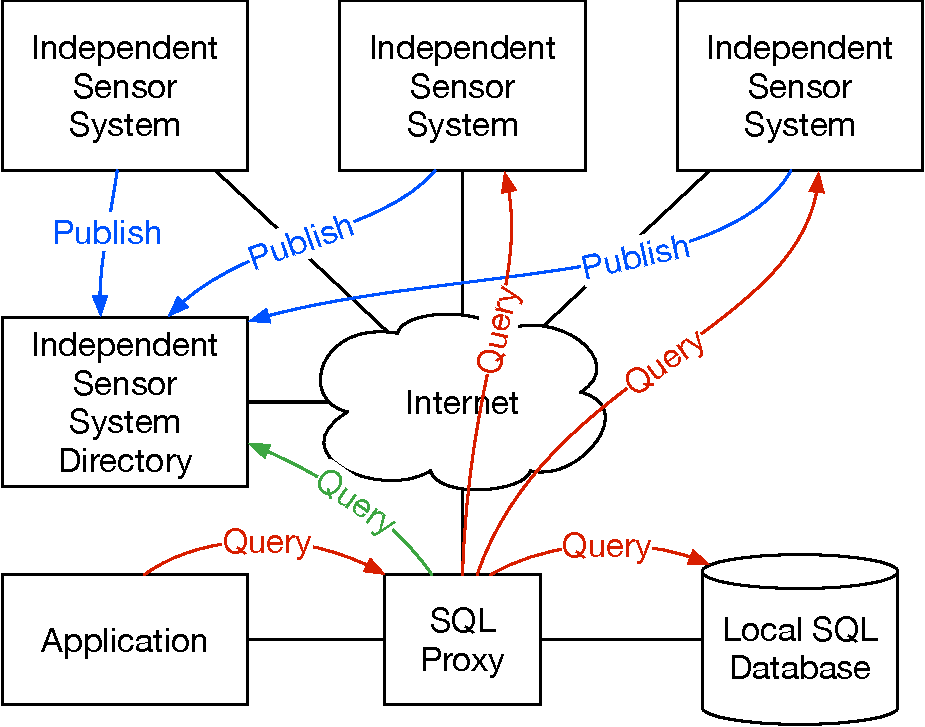
\includegraphics[width=0.8\linewidth]{figs/conceptual-diagram.pdf}
  \caption{Conceptual diagram}
  \label{fig:conceptual-diagram}
\end{figure}

Refer to Figure~\ref{fig:conceptual-diagram} for a conceptual diagram of the query processing architecture. To obtain the required measurement data, the application issues a SQL \textit{SELECT} query to a pre-configured SQL proxy. The proxy can be provided by the application's execution environment, e.g., the cloud infrastructure the application is running on.

If the SQL query does not refer to a virtual \textit{measurements} table or if it does not contain spatial predicates~\cite{sql-spatial,simple-feature-access}, the proxy forwards the query to a pre-configured local SQL database. The database is also provided by the application's execution environment. It contains geographic objects, application-specific data, and may also serve as a cache for previously obtained measurement data.

If the SQL query refers to the virtual \textit{measurements} table and contains spatial predicates, the proxy executes the query in a distributed manner. First, it retrieves the representations of relevant spatial objects from the local SQL database. Second, the proxy submits the representations to an Independent Sensor System Directory (ISSD). The ISSD returns a set of Independent Sensor Systems (ISSs) likely to have relevant measurement data. Third, the proxy transforms the original SQL query into sub-queries and forwards those to the ISSs. Finally, the proxy merges and aggregates partial results from the ISSs for the application.

Our architecture is designed to support queries over large geographic areas and the spatial objects involved in such queries could be quite complex\footnote{Measured by the number of points in the region's boundary polygon.}. For example, the boundary polygon for Morningside Heights neighborhood obtained from OpenStreetMaps has 89 points. The boundary polygon for Manhattan borough, the immediate enclosing spatial object, contains almost 1700 points.

To alleviate the need for the ISSD to process complex spatial objects, the SQL proxy runs a polygon simplification algorithm, similar to~\cite{song2011polygon}, on the spatial objects submitted to the ISSD. The algorithm must be carefully designed to fully contain the original polygon entirely\footnote{Violating this requirement may result in an incomplete ISS set, missing sensor measurement data, and incorrect results.}. This optimization may result in false positives, i.e., measurement data that should have been excluded from the result set. Thus, the SQL proxy must filter the data returned from ISSs using the original (not simplified) polygons. This important optimization shifts the burden of complex spatial object processing from the ISSD to the SQL proxy and thus the application executing the SQL query.

\section{Data Model}
\label{sec:data-model}

\subsection{Spatial Objects}
\label{sec:spatial-objects}

\textit{Discuss how spatial objects are stored in the local SQL database, what they represent, where they come from, and what kind of processing  must be performed on data obtained, e.g., from OpenStreetMaps}.

\subsection{Sensor Measurement Data}
\label{sec:sensor-measurements}

\textit{Discuss the design of the virtual measurements table, including how various types of measurements (discreet and continuous) are stored in the virtual table.}

\section{Event Notification}
\section{sec:event-notification}

\section{Conclusion}
\label{sec:conclusion}

\subsection{Future Work}
\label{sec:future-work}

Similar basic mechanism could work for updating some kinds of actuators (via SQL \textit{UPDATE}). Particularly, the reliability of the updates could be justified in the face of conflicts or failing actuator updates. The ACID semantics might be useful, or a model similar to \href{https://dl.acm.org/doi/pdf/10.1145/2491245}{Google Spanner}.

\bibliographystyle{IEEEtran}
\bibliography{bibs/references,bibs/rfc,bibs/db}
\end{document}
